\thispagestyle{fancy}
	
% 	\vspace{-2em} % Adjust vertical space as needed
% 	\begin{center}



% \addcontentsline{toc}{subsection}{Message of the Symposium Chair}    
% \subsection*{\textsc{Message of the Symposium Chair}}
% 	\end{center}

   
    
%     \begin{wrapfigure}{l}{0.3\textwidth}
% 		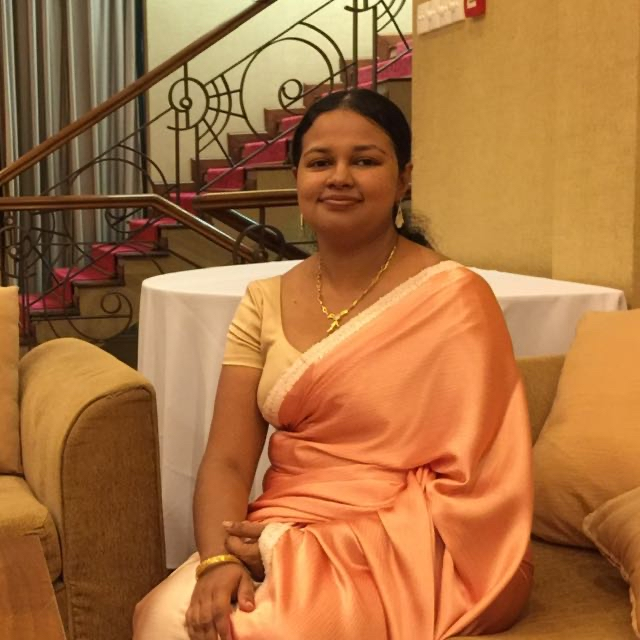
\includegraphics[width=0.3\textwidth]{Images/chair.jpeg}
% 	\end{wrapfigure}
% 	\vspace{2em} % Adjust vertical space as needed


\addmessage{Symposium Chair}{chair.jpeg}

	
As the Symposium Chair of IRS 2024 it is  an honour for me to welcome all of you to IRS 2024. This year, University of Vocational technology is very proudly hosting IRS 2024  under theme “Vocational Technology Education for Sustainable Greener Economy" . It is the 8\textsuperscript{th} research symposium organized by the university  and  IRS has become a tradition in the university and it has fostered a research culture in the university and it has been beneficial for  all of us to advance in our research careers.

This year’s theme marks an important responsibility that has being entrusted to University of Vocational Technology as the only university catering to TVET sector in the country.  With the whole world, Sri Lanka too is planning to steer our economy towards sustainable development and green economy. During this journey our  country will  need an empowered skillful work force who  can adopt to dynamic challenging situations and  TVET sector will be entrusted with building this  workforce.  We believe IRS 2024 will be an ideal platform to present research outputs and disseminate new knowledge that can empower the TVET sector professionals  to thrive and meet these new challenging goals.

The feedback we received for this symposium was beyond our expectations and we received a large number of research papers in  various fields that are aligning with our five tracks. All the papers were evaluated through blind review process by at least two subject experts and the feedback was given to the authors to improve the quality of their research work and the papers meeting the expected academic and research standards were selected for the presentations. On behalf of the program committee , I extend my heartiest gratitude towards all the reviewers who dedicated their valuable time and provided us the feedback required to maintain the academic standards of the symposium.  


Congratulations to all the authors on your achievement and we are looking forward to a productive day of disseminating knowledge and insightful discussions. I am confident that the proceedings of  IRS 2024 will inspire all of us to explore new research paths and conduct prominent research work in our respective fields.



% As the Symposium Chair of IRS 2024, it is an honour to welcome you all. This year, the University of Vocational Technology proudly hosts IRS 2024 under the theme “Vocational Technology Education for Sustainable Greener Economy.” This 8th research symposium has become a tradition, fostering a research culture and benefiting our careers.

% This year’s theme highlights the responsibility of the University of Vocational Technology as the only university catering to the TVET sector in the country. Sri Lanka is steering towards sustainable development and a green economy, requiring a skilled workforce. TVET will build this workforce. IRS 2024 is an ideal platform to present research in sustainable TVET, innovation, entrepreneurship, and sustainable practices in industrial, digital, and engineering technologies.

% We received a large number of research papers, evaluated through a blind review process by subject experts. Selected papers met academic and research standards. I extend gratitude to all reviewers for their valuable feedback.

% I thank the Vice Chancellor for guidance and mentorship, and all staff members for their dedication. Congratulations to all authors. We look forward to a productive day of knowledge dissemination and discussions. I am confident IRS 2024 will inspire new research paths and prominent work in our fields.

	% \vspace{1cm}
	% \noindent
    
Ms. P.M. Perera \\
Symposium Chair - International Research Symposium 2024 - UOVT


	\newpage
	